\documentclass[10pt]{article}

\PassOptionsToPackage{numbers, sort&compress}{natbib}

%\usepackage{changepage}

\usepackage{amsmath, amssymb, amsthm}
\usepackage{algorithm}
\usepackage{mathtools}
%\usepackage{caption}
%\usepackage{subcaption}
\usepackage{float}
\usepackage{framed}
\usepackage[noend]{algpseudocode}
\usepackage{enumitem}
\usepackage{tikz}
\usepackage{thmtools, thm-restate}

\usepackage[utf8]{inputenc} % allow utf-8 input
\usepackage[T1]{fontenc}    % use 8-bit T1 fonts
\usepackage[hidelinks]{hyperref}       % hyperlinks
\usepackage{url}            % simple URL typesetting
\usepackage{booktabs}       % professional-quality tables
\usepackage{amsfonts}       % blackboard math symbols
\usepackage{nicefrac}       % compact symbols for 1/2, etc.
\usepackage{microtype}      % microtypography
\usepackage{xcolor}         % colors
\usepackage{wrapfig}
\usepackage{tabularx}
\usepackage{makecell}

% Recommended, but optional, packages for figures and better typesetting:
\usepackage{graphicx}
\usepackage{subcaption}
\usepackage{multirow}
\usepackage{fancyhdr}
\usepackage[capitalize,noabbrev]{cleveref}

\renewcommand{\O}{\mathcal{O}}

\pagestyle{fancy}
\lhead{COMSC 312}
\rhead{Spring 2026}


\theoremstyle{definition}
\newtheorem{problem}{Problem}
\newenvironment{solution}{\begin{proof}[Solution]}{\end{proof}}

\title{Homework 4: Graphs}
\date{}

\begin{document}

\maketitle
\thispagestyle{fancy}

\noindent You may work in groups, but you must write solutions yourself. List your collaborators at the top of your submission. 

\vspace{1em}

\noindent \textbf{Instructions for submission:} Submit your homework as a single PDF file to the course Gradescope page. Either scan your \emph{legible} handwritten solutions or type them up in \LaTeX. 



\begin{problem}
    Consider the following graph $G$ with ten vertices:
    \begin{center}
    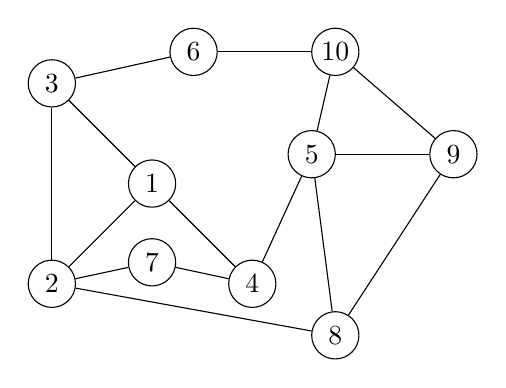
\begin{tikzpicture}[node distance={18mm}, main/.style = {draw, circle, minimum size=6mm, inner sep=0pt}] 
        \node[main] (1) {$1$};
        \node[main] (2) [below left of=1] {$2$};
        \node[main] (3) [above left of=1] {$3$};
        \node[main] (4) [below right of=1] {$4$};
        \node[main] (6) [right of=3,yshift=4mm] {$6$};
        \node[main] (7) [below of=1, yshift=8mm] {$7$};
        \node[main] (10) [right of=6] {$10$};
        \node[main] (5) [below of=10,xshift=-3mm,yshift=5mm] {$5$};
        \node[main] (9) [right of=5] {$9$};
        \node[main] (8) [below of=5,xshift=3mm,yshift=-5mm] {$8$};

        \draw (1) -- (2) (1) -- (3) (1) -- (4);
        \draw (2) -- (3); 
        \draw (2) -- (7);
        \draw (2) -- (8); 
        \draw (3) -- (6); 
        \draw (4) -- (5);
        \draw (4) -- (7); 
        \draw (5) -- (8); 
        \draw (5) -- (9);
        \draw (5) -- (10);
        \draw (6) -- (10);
        \draw (8) -- (9);
        \draw (9) -- (10);
    \end{tikzpicture}
    \end{center}

    \begin{enumerate}[label=(\alph*)]
        \item What is the distance between vertices $1$ and $8$?
        \item \textbf{BFS I} 
        \begin{enumerate}[label=(\roman*)]
            \item List the order in which the vertices are visited when we run a breadth-first search starting from vertex $1$. Assume that we visit neighbors in \emph{increasing} order of their labels.
            \item How many layers does the BFS tree have? \textbf{Hint}: $L_0$ counts as a layer.
            \item Which vertices are in $L_2$?
        \end{enumerate}

        \item \textbf{BFS II} 
        \begin{enumerate}[label=(\roman*)]
            \item List the order in which the vertices are visited when we run a breadth-first search starting from vertex $1$. Assume that we visit neighbors in \emph{decreasing} order of their labels.
            \item How many layers does the BFS tree have? 
            \item Which vertices are in $L_2$?
        \end{enumerate}
        
        \item \textbf{DFS}: List the order in which the vertices are visited (i.e. explored) when we run a depth-first search starting from vertex $1$. Assume that we visit neighbors in \emph{increasing} order of their labels.
    \end{enumerate}
\end{problem}

% \begin{solution}
%     This is a sample solution.
% \end{solution}

\begin{problem}
    In lecture, we showed that if a graph $G$ has an odd cycle, then it cannot be bipartite. We proved this using a coloring argument, where each of the two colors represents a partition. This showed that if a graph is bipartite, then it has no odd cycles. Prove the converse: if a graph $G$ has no odd cycles, then $G$ is bipartite. \textbf{Hint}: use the BFS tree to construct the two partitions into even layers and odd layers.
\end{problem}

% \begin{solution}
%     This is a sample solution.
% \end{solution}

\end{document}
